%!TEX encoding = UTF-8 Unicode
\documentclass[french]{article}



%% Langue et compilation

\usepackage[utf8]{inputenc}
\usepackage[T1]{fontenc}
\usepackage[french]{babel}

%% LISTE DES PACKAGES

\usepackage{mathtools}     % package de base pour les maths
\usepackage{amsmath}       % mathematical type-setting
\usepackage{amssymb}       % symbols speciaux pour les maths
\usepackage{textcomp}      % symboles speciaux pour el text
\usepackage{gensymb}       % commandes generiques \degree etc...
\usepackage{tikz}          % package graphique
\usepackage{wrapfig}       % pour entourer a cote d'une figure
\usepackage{color}         % package des couleurs
\usepackage{xcolor}        % autre package pour les couleurs
\usepackage{pgfplots}      % pacakge pour creer des graph
\usepackage{epsfig}        % permet d'inclure des graph en .eps
\usepackage{graphicx}      % arguments dans includegraphics
\usepackage{pdfpages}      % permet d'insérer des pages pdf dans le document
\usepackage{subfig}        % permet de creer des sous-figure
\usepackage{pst-all}       % utile pour certaines figures en pstricks
\usepackage{lipsum}        % package qui permet de faire des essais
\usepackage{array}         % permet de faire des tableaux
\usepackage{multicol}      % plusieurs colonnes sur une page
\usepackage{enumitem}      % pro­vides user con­trol: enumerate, itemize and description
\usepackage{hyperref}      % permet de creer des hyperliens dans le document
\usepackage{lscape}        % permet de mettre une page en mode paysage
\usepackage{lmodern}       % permet d'avoir certains "fonts" de bonen qualite
\usepackage{fancyhdr}      % Permet de mettre des informations en hau et en bas de page      
\usepackage[framemethod=tikz]{mdframed} % breakable frames and coloured boxes
\usepackage[top=1.5cm, bottom=1.5cm, left=2.5cm, right=2.5cm]{geometry} % donne les marges
\usepackage[font=normalsize, labelfont=bf,labelsep=endash, figurename=Fig.]{caption} % permet de changer les legendes des figures
\usepackage{lewis}
\usepackage{bohr}
\usepackage{chemfig}
\usepackage{chemist}

%% LIBRAIRIES

\usetikzlibrary{plotmarks} % librairie pour les graphes
\usetikzlibrary{patterns}  % necessaire pour certaines choses predefinies sur tikz
\usetikzlibrary{shadows}   % ombres des encadres
\usetikzlibrary{backgrounds} % arriere plan des encadres


%% MISE EN PAGE

\pagestyle{fancy}     % Défini le style de la page

\renewcommand{\headrulewidth}{1pt}      % largeur du trait en haut de la page
\fancyhead[L]{Seconde générale}         % info coin haut gauche
\fancyhead[R]{Lycée Jean Guéhenno}  % info coin haut droit

% bas de la page
\renewcommand{\footrulewidth}{1pt}      % largeur du trait en bas de la page
\fancyfoot[L]{G. \bsc{LE DOUDIC}}  % info coin bas gauche
\fancyfoot[R]{TP 4 : Famille chimique}                         % info coin bas droit


\setlength{\columnseprule}{1pt} 
\setlength{\columnsep}{30pt}



%% NOUVELLES COMMANDES 

\DeclareMathOperator{\e}{e} % permet d'ecrire l'exponentielle usuellement


\newcommand{\gap}{\vspace{0.15cm}}   % defini une commande pour sauter des lignes
\renewcommand{\vec}{\overrightarrow} % permet d'avoir une fleche qui recouvre tout le vecteur
\newcommand{\bi}{\begin{itemize}}    % begin itemize
\newcommand{\ei}{\end{itemize}}      % end itemize
\newcommand{\bc}{\begin{center}}     % begin center
\newcommand{\ec}{\end{center}}       % end center
\newcommand\opacity{1}               % opacity 
\pgfsetfillopacity{\opacity}

\newcommand*\Laplace{\mathop{}\!\mathbin\bigtriangleup} % symbole de Laplace

\frenchbsetup{StandardItemLabels=true} % je ne sais plus

\newcommand{\smallO}[1]{\ensuremath{\mathop{}\mathopen{}o\mathopen{}\left(#1\right)}} % petit o

\newcommand{\cit}{\color{blue}\cite} % permet d'avoir les citations de couleur bleues
\newcommand{\bib}{\color{black}\bibitem} % paragraphe biblio en noir et blanc
\newcommand{\bthebiblio}{\color{black} \begin{thebibliography}} % idem necessaire sinon bug a cause de la couleur
\newcommand{\ethebiblio}{\color{black} \end{thebibliography}}   % idem
%%% TIKZ


%% COULEURS 


\definecolor{definitionf}{RGB}{220,252,220}
\definecolor{definitionl}{RGB}{39,123,69}
\definecolor{definitiono}{RGB}{72,148,101}

\definecolor{propositionf}{RGB}{255,216,218}
\definecolor{propositionl}{RGB}{38,38,38}
\definecolor{propositiono}{RGB}{109,109,109}

\definecolor{theof}{RGB}{255,216,218}
\definecolor{theol}{RGB}{160,0,4}
\definecolor{theoo}{RGB}{221,65,100}

\definecolor{avertl}{RGB}{163,92,0}
\definecolor{averto}{RGB}{255,144,0}

\definecolor{histf}{RGB}{241,238,193}

\definecolor{metf}{RGB}{220,230,240}
\definecolor{metl}{RGB}{56,110,165}
\definecolor{meto}{RGB}{109,109,109}


\definecolor{remf}{RGB}{230,240,250}
\definecolor{remo}{RGB}{150,150,150}

\definecolor{exef}{RGB}{240,240,240}

\definecolor{protf}{RGB}{247,228,255}
\definecolor{protl}{RGB}{105,0,203}
\definecolor{proto}{RGB}{174,88,255}

\definecolor{grid}{RGB}{180,180,180}

\definecolor{titref}{RGB}{230,230,230}

\definecolor{vert}{RGB}{23,200,23}

\definecolor{violet}{RGB}{180,0,200}

\definecolor{copper}{RGB}{217, 144, 88}

%% Couleur des ref

\hypersetup{
	colorlinks=true,
	linkcolor=black,
	citecolor=blue,
	urlcolor=black
		   }

%% CADRES


% %%%%%%%%%% DEFINITION
% \newmdenv[tikzsetting={fill=definitionf}, linewidth=2pt, linecolor=definitionl, outerlinewidth=0pt, innertopmargin=5pt, innerbottommargin=5pt, innerleftmargin=5pt, innerrightmargin=5pt, leftmargin=0pt]{definition}

% \newmdenv[ tikzsetting={drop shadow={ shadow xshift=1ex, shadow yshift=-0.5em, fill=definitiono, opacity=1, every shadow } }, outerlinewidth=2pt, outerlinecolor=white, linecolor=white, innertopmargin=0pt, innerbottommargin=0pt, innerleftmargin=0pt, innerrightmargin=0pt]{ombredef}


% %%%%%%%%%% THEOREME

% \newmdenv[tikzsetting={fill=theof}, linewidth=2pt, linecolor=theol, outerlinewidth=0pt, innertopmargin=5pt, innerbottommargin=5pt, innerleftmargin=5pt, innerrightmargin=5pt, leftmargin=0pt]{theo}

% \newmdenv[ tikzsetting={drop shadow={ shadow xshift=1ex, shadow yshift=-0.5em, fill=theoo, opacity=1, every shadow } }, outerlinewidth=2pt, outerlinecolor=white, linecolor=white, innertopmargin=0pt, innerbottommargin=0pt, innerleftmargin=0pt, innerrightmargin=0pt]{ombretheo}


% %%%%%%%%%% METHODE

% \newmdenv[tikzsetting={fill=metf}, linewidth=2pt, linecolor=metl, outerlinewidth=0pt, innertopmargin=5pt, innerbottommargin=5pt, innerleftmargin=5pt, innerrightmargin=5pt, leftmargin=0pt]{met}

% \newmdenv[ tikzsetting={drop shadow={ shadow xshift=1ex, shadow yshift=-0.5em, fill=meto, opacity=1, every shadow } }, outerlinewidth=2pt, outerlinecolor=white, linecolor=white, innertopmargin=0pt, innerbottommargin=0pt, innerleftmargin=0pt, innerrightmargin=0pt]{ombremet}



%%%%%%%%%%% RQ

\newmdenv[tikzsetting={fill=remf}, linewidth=2pt, linecolor=remf, outerlinewidth=0pt, innertopmargin=5pt, innerbottommargin=5pt, innerleftmargin=5pt, innerrightmargin=5pt, leftmargin=0pt]{remarque}

\newmdenv[ tikzsetting={drop shadow={ shadow xshift=1ex, shadow yshift=-0.5em, fill=remo, opacity=1, every shadow } }, outerlinewidth=2pt, outerlinecolor=white, linecolor=white, innertopmargin=0pt, innerbottommargin=0pt, innerleftmargin=0pt, innerrightmargin=0pt]{ombreremarque}

%%%%%%%%%%% Cadre pour le titre

\tikzset{every shadow/.style={opacity=1}}

\global\mdfdefinestyle{doc}{backgroundcolor=white, shadow=true, shadowcolor=propositiono, linewidth=1pt, linecolor=black, shadowsize=5pt}
\global\mdfdefinestyle{titr}{backgroundcolor=metf, shadow=true, shadowcolor=propositiono, linewidth=1pt, linecolor=black, shadowsize=5pt}
\global\mdfdefinestyle{theo}{backgroundcolor=theof, shadow=true, shadowcolor=theoo, linewidth=1pt, linecolor=theol, shadowsize=5pt}
\global\mdfdefinestyle{prop}{backgroundcolor=theof, shadow=true, shadowcolor=propositiono, linewidth=1pt, linecolor=theol, shadowsize=5pt}
\global\mdfdefinestyle{def}{backgroundcolor=definitionf, shadow=true, shadowcolor=definitiono, linewidth=1pt, linecolor=definitionl, shadowsize=5pt}
\global\mdfdefinestyle{histo}{backgroundcolor=histf, shadow=true, shadowcolor=propositiono, linewidth=1pt, linecolor=black, shadowsize=5pt}
\global\mdfdefinestyle{avert}{backgroundcolor=white, shadow=true, shadowcolor=averto, linewidth=1pt, linecolor=avertl, shadowsize=5pt}
\global\mdfdefinestyle{met}{backgroundcolor=metf, shadow=true, shadowcolor=meto, linewidth=1pt, linecolor=metl, shadowsize=5pt}
\global\mdfdefinestyle{rem}{backgroundcolor=metf, shadow=true, shadowcolor=meto, linewidth=1pt, linecolor=metf, shadowsize=5pt}
\global\mdfdefinestyle{exo}{backgroundcolor=exef, shadow=true, shadowcolor=propositiono, linewidth=1pt, linecolor=exef, shadowsize=5pt}
\global\mdfdefinestyle{not}{backgroundcolor=definitionf, shadow=true, shadowcolor=propositiono, linewidth=1pt, linecolor=black, shadowsize=5pt}
\global\mdfdefinestyle{proto}{backgroundcolor=protf, shadow=true, shadowcolor=proto, linewidth=1pt, linecolor=protl, shadowsize=5pt}

%%%%%%
\definecolor{cobalt}{rgb}{0.0, 0.28, 0.67}
\definecolor{applegreen}{rgb}{0.55, 0.71, 0.0}

\usepackage{tcolorbox}
  \tcbuselibrary{most}
  \tcbset{colback=cobalt!5!white,colframe=cobalt!75!black}



\newtcolorbox{definition}[1]{
	colback=applegreen!5!white,
  	colframe=applegreen!65!black,
	fonttitle=\bfseries,
  	title={#1}}
\newtcolorbox{Programme}[1]{
	colback=cobalt!5!white,
  	colframe=cobalt!65!black,
	fonttitle=\bfseries,
  	title={#1}}  

\newtcolorbox{Exercice}[1]{
  colback=cobalt!5!white,
  colframe=cobalt!65!black,
  fonttitle=\bfseries,
  title={#1}}  

  \newtcolorbox{Protocol}[1]{
  colback=cyan!5!white,
  colframe=cyan!65!black,
  fonttitle=\bfseries,
  title={#1}}  

\newtcolorbox{Resultat}[1]{
	colback=theof,%!5!white,
	colframe=theoo!85!black,
  fonttitle=\bfseries,
	title={#1}} 	


\def\width{12}
\def\hauteur{5}

\setlength{\parskip}{0pt}%
\setlength{\parindent}{18pt}


%% MODIFICATION DE CHAPTER  
\makeatletter
\def\@makechapterhead#1{%
  %%%%\vspace*{50\p@}% %%% removed!
  {\parindent \z@ \raggedright \normalfont
    \ifnum \c@secnumdepth >\m@ne
        \huge\bfseries \@chapapp\space \thechapter
        \par\nobreak
        \vskip 20\p@
    \fi
    \interlinepenalty\@M
    \Huge \bfseries #1\par\nobreak
    \vskip 40\p@
  }}
\def\@makeschapterhead#1{%
  %%%%%\vspace*{50\p@}% %%% removed!
  {\parindent \z@ \raggedright
    \normalfont
    \interlinepenalty\@M
    \Huge \bfseries  #1\par\nobreak
    \vskip 40\p@
  }}
  
  \newcommand{\isotope}[3]{%
     \settowidth\@tempdimb{\ensuremath{\scriptstyle#1}}%
     \settowidth\@tempdimc{\ensuremath{\scriptstyle#2}}%
     \ifnum\@tempdimb>\@tempdimc%
         \setlength{\@tempdima}{\@tempdimb}%
     \else%
         \setlength{\@tempdima}{\@tempdimc}%
     \fi%
    \begingroup%
    \ensuremath{^{\makebox[\@tempdima][r]{\ensuremath{\scriptstyle#1}}}_{\makebox[\@tempdima][r]{\ensuremath{\scriptstyle#2}}}\text{#3}}%
    \endgroup%
  }%

\makeatother


%%
%% DEBUT DU DOCUMENT
%%

\begin{document}
\tikzset{every shadow/.style={opacity=1}}

\global\mdfdefinestyle{doc}{backgroundcolor=white, shadow=true, shadowcolor=propositiono, linewidth=1pt, linecolor=black, shadowsize=5pt}
\global\mdfdefinestyle{titr}{backgroundcolor=titref, shadow=true, shadowcolor=propositiono, linewidth=1pt, linecolor=black, shadowsize=5pt}
\global\mdfdefinestyle{theo}{backgroundcolor=theof, shadow=true, shadowcolor=theoo, linewidth=1pt, linecolor=theol, shadowsize=5pt}
\global\mdfdefinestyle{prop}{backgroundcolor=theof, shadow=true, shadowcolor=propositiono, linewidth=1pt, linecolor=theol, shadowsize=5pt}
\global\mdfdefinestyle{def}{backgroundcolor=definitionf, shadow=true, shadowcolor=definitiono, linewidth=1pt, linecolor=definitionl, shadowsize=5pt}
\global\mdfdefinestyle{histo}{backgroundcolor=histf, shadow=true, shadowcolor=propositiono, linewidth=1pt, linecolor=black, shadowsize=5pt}
\global\mdfdefinestyle{avert}{backgroundcolor=white, shadow=true, shadowcolor=averto, linewidth=1pt, linecolor=avertl, shadowsize=5pt}
\global\mdfdefinestyle{met}{backgroundcolor=metf, shadow=true, shadowcolor=meto, linewidth=1pt, linecolor=metl, shadowsize=5pt}
\global\mdfdefinestyle{rem}{backgroundcolor=metf, shadow=true, shadowcolor=meto, linewidth=1pt, linecolor=metf, shadowsize=5pt}
\global\mdfdefinestyle{exo}{backgroundcolor=exef, shadow=true, shadowcolor=propositiono, linewidth=1pt, linecolor=exef, shadowsize=5pt}
\global\mdfdefinestyle{not}{backgroundcolor=definitionf, shadow=true, shadowcolor=propositiono, linewidth=1pt, linecolor=black, shadowsize=5pt}
\global\mdfdefinestyle{proto}{backgroundcolor=protf, shadow=true, shadowcolor=proto, linewidth=1pt, linecolor=protl, shadowsize=5pt}

%%%%%%

\begin{center}
	\begin{mdframed}[style=titr, leftmargin=55pt, rightmargin=55pt, innertopmargin=8pt, innerbottommargin=8pt, innerrightmargin=10pt, innerleftmargin=10pt]
		
		
		\begin{center}
			\Large{\textbf{Chapitre 1: Émission et perception d'un son}} \\
			\large{\textbf{TP1: \og{}Autour du son\fg{}  et TP2: \og{}Vitesse du son\fg{}}}
		\end{center}
	\end{mdframed}
\end{center}
\section*{Objectifs du programme}
\begin{figure}[!ht]
	\centering
	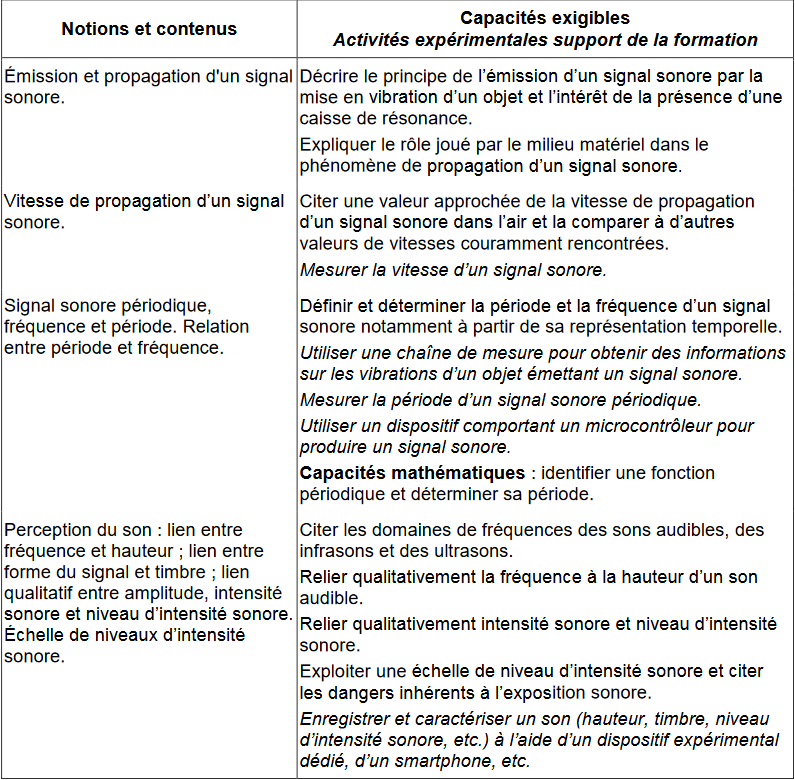
\includegraphics[width=1\textwidth]{./figures/BO.png}
\end{figure}

\begin{mdframed}[style=doc, leftmargin=0pt, rightmargin=0pt, innertopmargin=8pt, innerbottommargin=8pt, innerrightmargin=10pt, innerleftmargin=10pt]
		\noindent\textbf{Exercices}\medskip

		\begin{itemize}
			\item fréquence et période : Exercices 5,8 p.262 du Livre scolaire.
			\item niveaux sonores : Exercices 12, 14 p262
			\item vitese du son : Exercices  7, 10 p262
			\item Pour se préparer au devoir surveillé : Exercices 17p262, 23p266, 26p267
			
		\end{itemize}
\end{mdframed}
\clearpage
\section{Émission et propagation d'un son}

Qu'est-ce que le son ? Comment se propage-t-il ? À mettre en lien avec l'activé expérimentale du TP1
.



\subsection{Émission d'un son}

Un son est produit par la mise en \textbf{vibration} rapide d'un objet. Comme par exemple les cordes d'une guitare, les ailes d'un insecte ou les feuilles d'un arbre secouées par le vent. 

\begin{figure}[ht!]
	\centering
	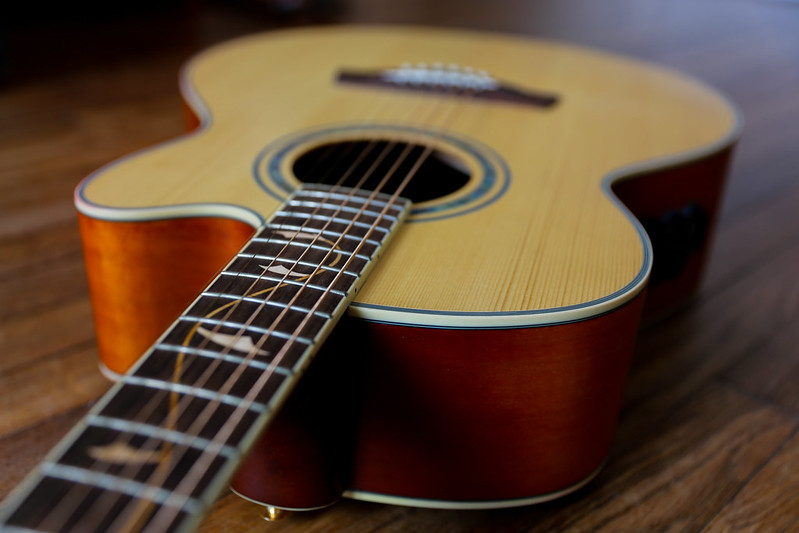
\includegraphics[width=.25\textwidth]{./figures/guitare.jpg}\hfill
	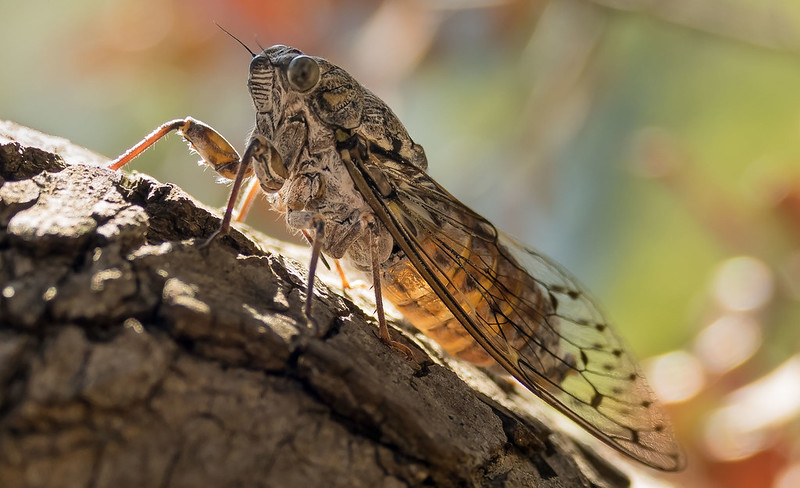
\includegraphics[width=.28\textwidth]{./figures/cigale.jpg}\hfill
	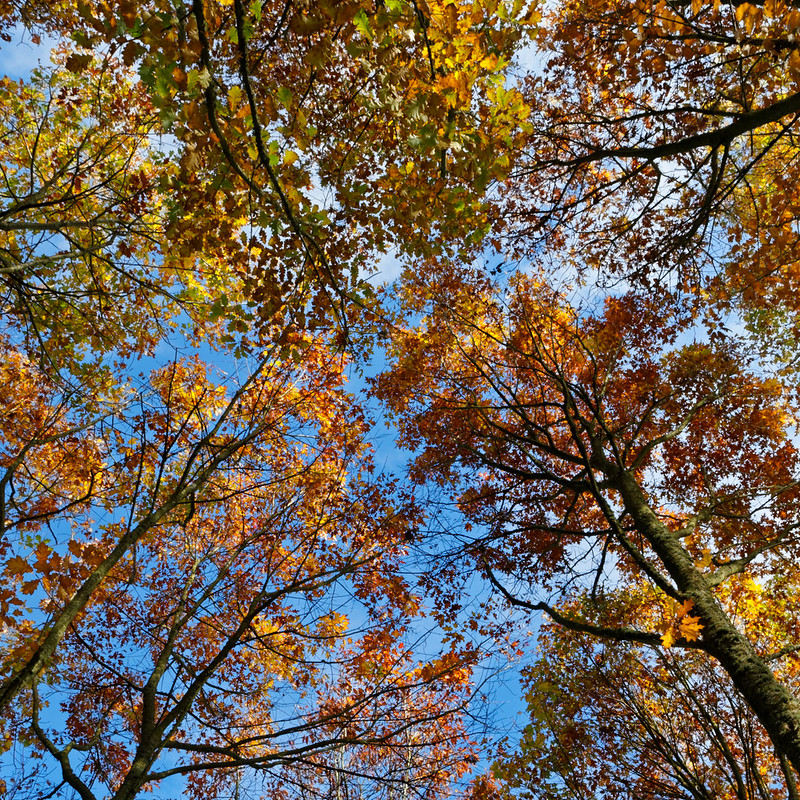
\includegraphics[width=.15\textwidth]{./figures/cimearbres.jpg}
	\caption{Une guitare, une cigale et la cime des arbres}
\end{figure}

Plus la surface mise en vibration est grande, plus le son sera fort. D'où l'intérêt d'utiliser des \textbf{caisses de résonance}. Une caisse de résonance \textbf{amplifie} et \textbf{filtre} les sons. On distinguera la production d'un son et d'un bruit par l'aspect \textbf{périodique} de l'onde sonore. On peut produire un son à une fréquence précise à l'aide d'un diapason frappé par un marteau. À l'oeil nu les vibrations peuvent être imperceptibles, on peut les mettre en évidence en plongeant une extrémité du diapason dans un verre d'eau par exemple. Lorsque l'on place le diapason sur une caisse de résonance appropriée le son est amplifié. (voir \url{https://www.youtube.com/watch?v=YRv4POv5jh4&t=23s&ab_channel=Unisciel})

\subsection{Propagation du son}

On entend un son en étant à distance de la source qui l'a crée, le son s'est donc \textbf{propagé} entre l'émetteur et le récepteur, dans l'air ou dans un autre milieu.\smallskip 

%\textbf{Que se passe-t-il si on fait le vide ? } (activité expérimentale réalisée par le professeur)

\begin{figure}[ht!]
	\centering
	\caption{\textbf{Que se passe-t-il lorsqu'on fait le vide ? }}
	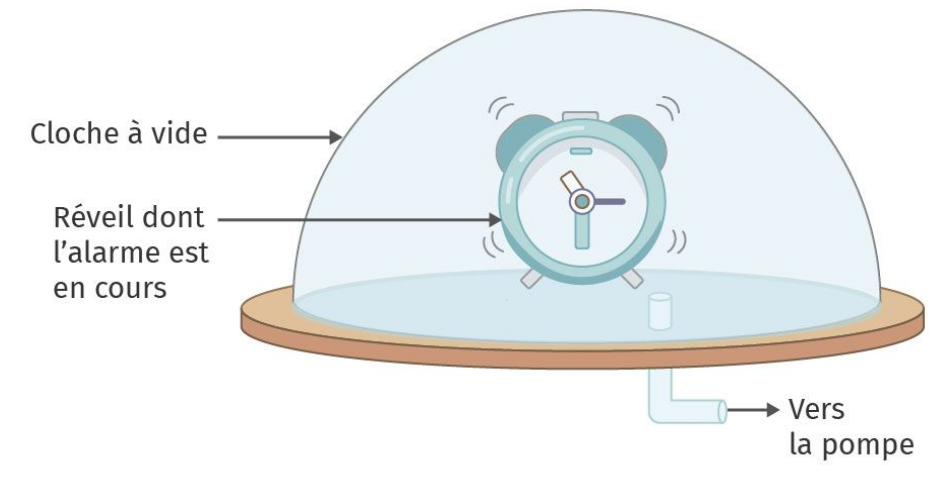
\includegraphics[width=.4\textwidth]{./figures/SonsDansUneClocheAVide.png}\hspace{2cm}
	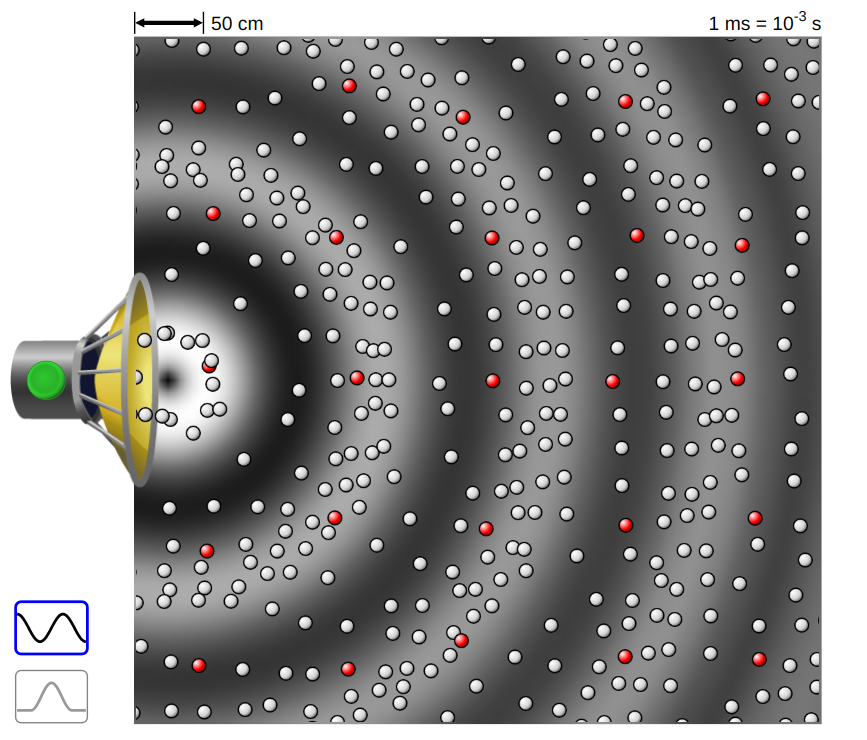
\includegraphics[width=.25\textwidth]{./figures/PropagationDunSon.png}\hfill
\end{figure}
\begin{definition}{Décrivez et interprétez les résultats expérimentaux }
	%\vspace{2.8cm}
	Un signal sonore est un phénomène de déplacement d'une perturbation de proche en proche dans un milieu matériel et sans transport effectif de matière. L'onde sonore nécessite un support matériel pour se déplacer, comme par exemple les molécules qui composent l'air, le bois, le métal, l'eau ou tout autre matériau.
\end{definition}
\begin{center}
\textbf{Lorsqu'on fait le vide le son ne se propage plus !\footnote{Animation: \url{https://phet.colorado.edu/sims/html/waves-intro/latest/waves-intro_fr.html}} }\smallskip
\end{center}
La perturbation a l'origine de la propagation est caractérisée par une vibration des molécules du milieu autour de leur \textbf{position d'équilibre} (ou état de repos).\bigskip 

Le mécanisme de propagation du son est réalisé en trois étapes que l'on peut résumé de la façon suivante: 

\begin{definition}{Les quatre étapes du mécanisme de propagation du son}
	% \vspace{3cm}

\begin{enumerate}
	\item La source mécanique crée une perturbation, qui se traduit par une variation de pression dans le milieu.
	\item Cette variation de pression provoque des micro-déplacements des molécules du milieu.
	\item Les molécules se heurtent entre elles, ce qui transmet la perturbation à leurs voisines.
\item Une fois la perturbation passée les molécules reviennent à leur position initiale.
\end{enumerate}
\end{definition}


\section{Des sons particuliers: les sons périodiques}

Certains sons sont constitués d'un motif qui se répète périodiquement, on parle de \textbf{sons périodiques}. Ils sont notamment caractérisés par la \textbf{fréquence} à laquelle se répètent les motifs.

 
\subsection{Hauteur d'un son}
La \textbf{hauteur du son}, c'est à dire s'il est aigu ou grave est lié à la \textbf{fréquence}. Plus la fréquence est grande plus le son est aigüe. A contrario, plus la fréquence est faible plus le son est grave. 

\begin{definition}{La fréquence et la période}
%\vspace{2.5cm}
La fréquence, notée $f$, d'un son est liée à la période $T$. C'est l'inverse de la periode. Mathématiquement la relation entre $f$ et $T$ s'écrit: 

\begin{equation}
	f = \dfrac{1}{T}
\end{equation}
La fréquence est l'inverse d'un temps, on l'exprime en \textbf{Hertz} (Hz) ce qui correspond à $1/s$ ou $s^{-1}$.
\end{definition}

\begin{wrapfigure}[10]{r}{.5\textwidth}%[ht!]
	\centering
	\vspace{-1cm}
	\includegraphics[width=.5\textwidth]{./figures/Deuxsignauxdifférents.png}
	\caption{Même fréquence mais un timbre différent.}
\end{wrapfigure}
\subsection{Le timbre}

En musique, des sons de même \textbf{hauteur} représentent la même note, par exemple un La3 si la fréquence du son est de $440 Hz$. Pourtant, même si deux instruments jouent la même note, ils sont différentiables et identifiables à l'oreille. On dit que leur \textbf{timbre} est différent. \textbf{Le timbre d'un son} est l'ensemble des caractéristiques du signal permettant de distinguer ce son d'un autre de même hauteur (ou même fréquence). Le timbre est lié à la forme du son.\medskip


\begin{Exercice}{Exercices}
	Savoir faire:
	\begin{enumerate}
		\item Déterminer une période à partir d'un graphique;
		\item Convertir des milisecondes en secondes;
		\item Calculer la fréquence d'un signal
	\end{enumerate}
	Exercices 5,8 p.262 du Livre scolaire.
\end{Exercice}

\section{Le son et l'oreille}


Lorsque l'onde sonore arrive à nos oreilles, d'un côté du tympan on aura une accumulation de molécules (plus de chocs) ce qui induit une force sur la membrane du tympan et son déplacement. Mais pas pour tous les types de sons !

\begin{wrapfigure}[4]{r}{.5\textwidth}
	\centering
	\includegraphics[width=.5\textwidth]{./figures/FréquencesAudibles.png}
	\caption{Domaine des fréquences audibles}
\end{wrapfigure}

\subsection{Le domaine des fréquences audibles}

L'oreille humaine ne perçoit que certaines fréquences sonores. Lesquelles ?
\begin{definition}{Domaine des fréquences audibles}
%\vspace{2.5cm}
Un son trop grave ou trop aigüe ne sera pas entendu. Le domaine de fréquence des sons audibles est compris entre \textbf{20 Hz et 20 kHz}. Ces valeurs peuvent varier d'un individu à l'autre et le domaine des fréquences audibles se réduit avec l'âge. En dessous de 20 Hz on se situe dans le domaine des \textbf{infrasons}. Au delà des 20 kHz on parle des \textbf{ultrasons}.
\end{definition}
\subsection{Intensité et niveaux sonores} 
% \begin{wrapfigure}[12]{r}{.5\textwidth}
% 	\centering
% 	\vspace{-1cm}
% 	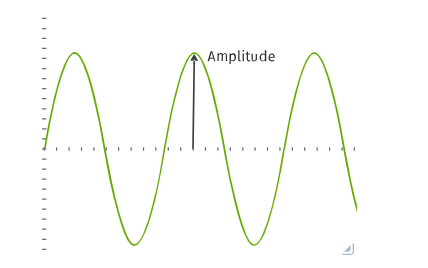
\includegraphics[width=.4\textwidth]{./figures/amplitude.png}
% 	\caption{Amplitude de l'onde sonore [le livre scolaire]}
% \end{wrapfigure}

L'\textbf{amplitude} du son correspond au maximum d'intensité que peut atteindre le signal sonore. Un son est deux fois plus intense si la source vibre avec une amplitude deux fois plus grande. Pourtant il ne sera pas perçu deux fois plus fort par l'oreille. L'oreille ne réagit \textbf{pas proportionnellement} à l'intensité de l'onde sonore, car elle est sensible à une gamme limitée de pressions. À partir d'une certaine intensité, elle ne peut plus distinguer les différences de pression.\bigskip

Pour modéliser ces observations expérimentales, on définit le \textbf{niveau d'intensité sonore} noté $L$ et exprimer en décibel (dB). On peut mesurer le niveau d'intensité sonore à l'aide d'un \textbf{sonomètre}.\medskip

% \vspace{1cm}
\textbf{Remarque:} lorsque le son est deux fois plus fort, le niveau d'intensité sonore augmente de 3 dB.


\subsection{Perception des sons par l'oreille}

L'onde sonore peut présenter un danger pour l'oreille, si son niveau d'intensité sonore est trop élevé. Le niveau 0 dB est le niveau minimum pour lequel l'oreille peut détecter le son. En dessous de ce niveau, l'oreille ne pourra pas entendre le son.Au delà d'un certain niveau, la vibration peut endommager l'oreille définitivement. On dit que le seuil de douleur correspond à un niveau de 120 dB.
\begin{figure}[ht!]%[3]{l}{.6\textwidth}%[ht!]
	\centering
	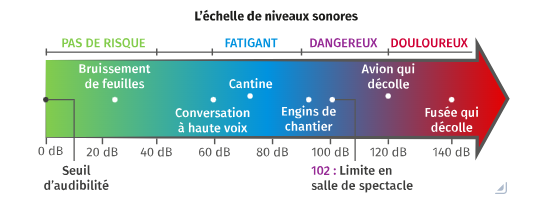
\includegraphics[width=.8\textwidth]{./figures/echelledesniveauxsonores.png}
	% \caption{Échelle des niveaux sonores [Le livre scolaire]}
\end{figure}
\begin{Exercice}{Exercices sur l'intensité sonore}
	Savoir Faire : 
	\begin{itemize}
		\item Lire un graphique de niveaux d'intensité sonore;
	\end{itemize}
	Exercices 12, 14 p262
\end{Exercice}
\clearpage
\section{Vitesse de propagation du son}
Voir l'activé expérimentale voir le TP2 \og{}Mesure de la vitesse du son dans l'air et dans l'eau\fg{}.
\begin{definition}{La vitesse du son}

	La vitesse du son correspond au rapport entre la distance $d$ parcourue par l'onde sonore et le temps $\Delta t$ qu'elle a mis à parcourir cette distance. 
\begin{equation}
	v = \dfrac{d}{\Delta t}
\end{equation}

La vitesse $v$ est donnée en mètres par secondes ($\rm m/s$ ou $\rm m\cdot s^{-1}$), la distance $d$ est en mètres (m) et le temps entre deux instants $\Delta t= t_2- t_1$ est donné en secondes (s).
\end{definition}

\begin{table}[ht!]
	\centering
	\begin{tabular}{|c|c|c|c|c|}
	\hline
	\textbf{Milieu}               & Air & Eau liquide & Verre & Acier \\ \hline
	$v~(\rm m \cdot s^{-1})$ & 340 & 1500        & 5300  & 5800  \\ \hline
	\end{tabular}
	\caption{Vitesse du son en fonction du milieu à $T=20^\circ \rm C$}
\end{table}
La vitesse de propagation d'une onde sonore dépend à la fois du milieu matériel et de sa température. Plus le milieu est dense, plus la vitesse de propagation sera grande. Et plus la température du milieu est grande plus la vitesse du son est importante.\medskip

\begin{Exercice}{Exercice sur la vitesse du son}
	Savoir Faire :
	\begin{itemize}
		\item Savoir calculer une vitesse, un temps ou une distance à partir des informations données;
		\item convertir une vitesse en "m/s" en "km/h"
	\end{itemize}
	Exercices 7, 10 p262
\end{Exercice}
% \section{Devoirs à la maison}

% Exercices à chercher à la maison : 17p268 et 23p266.








 
\end{document}

%%
%% FIN DU DOCUMENT
%%
